\chapter{Introducción}\label{cha:introduccion}

	\section{Presentación del Documento}

		El presente informe describe el proyecto de desarrollo de Kingdom of Hatred, un videojuego en dos dimensiones con niveles generados proceduralmente detallando tanto los objetivos que se pretenden alcanzar con el proyecto, como las fases, actividades y recursos necesarios para llevarlo a cabo.

		El contenido de este documento se estructura en torno a los siguientes apartados:

		\begin{itemize}
			\item \textbf{Introducción:}
				
			Definición del contenido del documento, resumen del estado del arte y motivación.
			
			\item \textbf{Objetivos del proyecto:}
				
			Establecimiento de los objetivos del proyecto, su alcance y las tareas a realizar.
			
			\item \textbf{Especificación de requisitos:}

			Descripción de los requisitos del proyecto, analizados desde distintos puntos de vista.

			\item \textbf{Especificación del diseño:}
			
			Descripción de la solución elegida y cómo ha sido aplicada.

			\item \textbf{Consideraciones de la implementación:}

			Descripción de los aspectos más destacables de la implementación.

			\item \textbf{Plan de pruebas:}

			Definición del plan de pruebas utilizado para garantizar la calidad del producto.

			\item \textbf{Manual de usuario:}

			Descripción del uso del producto desarrollado al usuario.

			\item \textbf{Incidencias:}

			Descripción de los problemas encontrados en el desarrollo y cómo de han solucionado.

			\item \textbf{Conclusiones:}

			Análisis de los objetivos alcanzados y consideraciones adicionales.
		\end{itemize}

	\section{Estado del arte y motivación}

		La industria de los videojuegos es el sector económico involucrado en el desarrollo, la distribución, la mercadotecnia, la venta de videojuegos y del hardware asociado. Engloba a docenas de disciplinas de trabajo y emplea a miles de personas alrededor del mundo.

		Esta ha mantenido en los últimos años su posición como principal industria de ocio audiovisual e interactivo, con una cuota de mercado muy superior a la del cine y la música. Por esta razón, enfocar una carrera profesional orientada al desarrollo de videojuegos es cada vez una opción más viable y habitual. En el pasado el desarrollo de videojuego era algo casi exclusivo de grandes empresas, ya que las herramientas necesarias para ello eran escasas y no estaban al alcance de todos. Sin embargo, en los últimos años estas se han hecho mucho más accesibles y eso ha hecho que aparezcan muchos desarrolladores nuevos, con lo cual la competitividad en el mercado es bastante grande.

		\subsubsection{Motores de videojuegos}

			Un motor de videojuego es un término que hace referencia a una serie de librerías de programación que permiten el diseño, la creación y la representación de un videojuego. Del mismo modo existen motores de juegos que operan tanto en consolas de videojuegos como en sistemas operativos. La funcionalidad básica de un motor es proveer al videojuego de un motor de renderizado para los gráficos 2D y 3D, motor físico o detector de colisiones, sonidos, scripting, animación, inteligencia artificial, redes, streaming, administración de memoria y un escenario gráfico.

			Entre los motores disponibles, se pueden diferenciar dos tipos: los que ofrecen editor visual y los que no.

			Los primeros son los más conocidos y utilizados por su sencillez y curva de aprendizaje. Estos motores habitualmente dan una base funcional para un juego, en el que la arquitectura del software ya está definida, y el usuario se limita a añadir elementos al juego, delegando en el motor el cometido de gestionarlos. Consecuentemente, estos motores son muy flexibles y pueden ser utilizados para crear prácticamente cualquier tipo de juego, pero tiene la debilidad de que la eficiencia no es siempre la máxima. Ejemplos de este tipo de motores podrían ser: Unity3D, Unreal Engine, CryEngine... Dado que uno de los objetivos fundamentales del proyecto es aprender a desarrollar videojuegos, se ha decidido no utilizar un motor de este tipo, ya que se pierde en gran medida el control sobre el software.

			Por otro lado existen otros motores que no cuentan con editor visual, de forma que en términos sencillos proveen al usuario con una \acrshort{api} para lo necesario en la realización de un videojuego. Estas alternativas conllevan un aumento muy grande de la carga de trabajo, pero tienen la ventaja de que los desarrolldores tienen el control total de lo que ocurre en cada parte del software, y al no tener una arquitectura preestablecida, pueden adaptarla al juego que se está creando, de forma que se consiga la mayor eficiencia. Entre los motores disponibles de este tipo se pueden nombrar \acrshort{sfml}, \acrshort{sdl} o libGDX. Para este proyecto se ha decidido usar un motor de este tipo, en concreto \acrshort{sfml}.

		\subsubsection{Desarrollos AAA y desarrollos independientes}

			En la industria del desarrollo de videojuegos, se conocen como AAA o triple A los desarrollos que cuentan con los más altos niveles de presupuesto y promoción para su realización. Por tanto, se espera que un título considerado AAA sea de una gran calidad y que sus ventas sean inmensas. Estos desarrollos son llevados a cabo por empresas de la industria ya establecidas como \acrshort{ea}~\cite{ea}, Ubisoft~\cite{ubisoft}, Valve~\cite{valve} y otras, aunque también existen casos de desarrollos de este tipo en empresas jóvenes gracias a la presencia de un inversor.

			Por otro lado, existen los desarrollos independientes, los cuales están en pleno auge desde hace unos pocos años. Estos cuenta con un presupuesto mucho más limitado, y la fuerza de producción suele ser la de un equipo de pocas personas. Actualmente, estos equipos se basan en créditos para llevar a cabo sus proyectos, aunque últimamente la financiación colectiva está cogiendo mucha fuerza. Los equipos están formados tanto por profesionales de la industria que han querido dar rienda suelta a su creatividad con un proyecto propio como por aficionados a videojuegos que aspiran a poder trabajar en el sector. Uno de los grandes problemas de los desarrollos independientes es que, al haber muchísismos equipos de desarrollo, la competitividad es grandísima, y solo unos pocos consiguen hacerse un hueco a un nivel más profesional.

		\subsubsection{\acrshort{rpg}s de acción}

			El juego que se va a desarrollar pertenece al género de los juegos de rol de acción. Estos juegos comparten muchas características con los juegos de rol tradicionales, pero su pricipal diferencia está en que ofrecen combates en tiempo real. Se ha elegido este género porque, además de que el alumno es un gran aficionado, supone un reto extra a la hora de desarrollar, ya que es necesario que la aplicación tenga en todo momento un respuesta en tiempo real y se han de gestionar adecuadamente todas las entidades para conseguirlo.

			La principal inspiración del juego ha sido la saga \textit{The Legend of Zelda}~\cite{zelda}, en particular la última entrega que se lanzó para \acrshort{gba}, subtitulada \textit{The Minish Cap}. Como otras influencias se pueden mencionar \textit{Hyper Light Drifter}, \textit{Sword of Mana} o \textit{Hero Siege}. En los últimos años este género ha ganado mucha fuerza, en gran parte gracias al más que notable salto que dió a las tres dimensiones, el cual atrajo a muchos nuevos jugadores. Sin embargo, los juegos en dos dimensiones han quedado ligeramente relegados, y lo más habitual es que sean desarrollados por empresas independientes o para consolas portátiles.

			\begin{figure}[!htp]
				 \centering
				 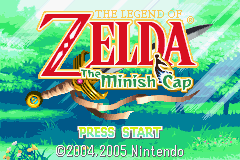
\includegraphics{fig/zelda}
				 \caption{Pantalla de inicio de \textit{The Legend of Zelda The Minish Cap}}
				 \label{fig:zelda}
			\end{figure}

			\FloatBarrier

		\subsubsection{Motivación}

			Este proyecto nace de la afición a los productos de entretenimiento digital y a la creación de los mismos, en concreto, al género de los juegos en dos dimensiones. El proyecto va a consistir en el desarrollo de una demo técnica de un juego de este tipo, desde el análisis de requisitos, diseño del juego y del software y su implementación. Además, los niveles del juegos tendrán que ser generados proceduralmente, así que se deberán implementar algoritmos adecuados para estos propósitos, junto con los demás requisitos típicos de un software tradicional (usabilidad, estabilidad...). El resultado principal consistirá en una demo de calidad, especialmente en el apartado de software, que pudiese competir con productos similares del mercado, además de servir como experiencia de aprendizaje para el desarrollo de futuros proyectos de esta índole.
